\documentclass[a4paper,11pt]{article}
\usepackage[utf8]{inputenc}
\usepackage[italian]{babel}
\usepackage[maxbibnames=99,backend=bibtex]{biblatex}
\usepackage{hyperref}
\usepackage{listings}
\usepackage{color}
\usepackage{graphicx}

\addbibresource{ref.bib}
\graphicspath{ {images/} }

% define the title
\author{Luigi Leonardi}
%\pagestyle{headings}

\title{Tirocinio su Posit}
\date{}


\definecolor{mygreen}{rgb}{0,0.6,0}

\lstset{  
	numbers=left,
	numbersep=5pt,
	commentstyle=\color{mygreen},
	keywordstyle=\color{blue}\ttfamily,
	stringstyle=\color{red}\ttfamily  
}


%link cliccabili
\hypersetup{colorlinks=true, linktoc=all,  linkcolor=black,citecolor=black}

\begin{document}
	% generates the title
	\maketitle
	% insert the table of contents
	\tableofcontents
	
%	\cite{epfl1}
	

\newpage
	\section{Introduzione}
	\subsection{Posit}

	Il Posit è un formato di numero in virgola mobile ideato da John Gustafson, in alternativa allo standard IEEE 754. L'idea di base è fondamentalmente la stessa, anche nei Posit è presente un bit per il segno, dei bit per l'esponente e dei bit per la mantissa, le principali differenze consistono nella presenza di un "super esponente" o regime e nel non avere un numero di bit fissato per quest'ultimo e per la mantissa. \\
	\begin{figure}[h]
	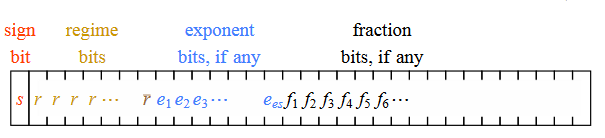
\includegraphics[scale=0.8]{posit}
	\centering
	\caption{"Formato Posit"}
	\end{figure}Il vantaggio nell'avere un super esponente, la cui lunghezza non è definita, permette di ottenere un range di numeri molto più flessibile, il suo contributo è pari a $2^{2^{es}}$ con es il numero di bit dell'esponente\footnote{L'esponente è l'unico campo ad avere una dimensione fissa}, permettendo quindi una riduzione del numero di bit assegnati a quest'ultimo campo oppure un incremento di range.\newline Questi bit di regime non sono altro che una sequenza di cifre binarie identiche, terminate dal complemento di esse. \newline Ad esempio: 0001 rappresenta -3, dove 3 è il numero degli 0 ed 1 è il terminatore.\footnote{Regimi che iniziano per 0 sono negativi, per 1 invece sono positivi. Lo 0 è rappresentato come 10}\cite{epfl1}
	
	\subsection{Note sui Test}
	Tutti i test svolti sui Posit sono stati effettuati sfruttando la libreria in C++ BFP\cite{libbfp} 
	implementando, dove necessario, le funzionalità mancanti.\newline I Posit scelti sono stati a 32/64 bit, con 0 bit di esponente\footnote{Ha senso non utilizzare bit di esponente, in quanto si sfrutta il super esponente}, dove non specificato diversamente.
	
%	\subsection{Cippi}
%	\ldots{} ora e' in distilleria.
\newpage
\section {Test su Moltiplicazione}
\subsection{Accuratezza}

Questo test vuole dimostrare che a parità di bit utilizzati, 32 in questo caso, i Posit risultano essere più precisi nel rappresentare i risultati di prodotti, rispetto ad un Float in precisione singola.\\
In questo particolare caso sono stati impiegati Posit [32,3], ossia 32 bit totali, di cui 3 di esponente.
\subsubsection{Svolgimento}
Il test consiste nel creare 9 array, 6 per gli operandi e 3 per i risultati, di una dimensione compresa nell'ordine dei milioni: \begin{itemize}
	\item 3 di Posit [32,3]
	\item 3 di Float a 32 bit 
	\item 3 di Double a 64 bit come riferimento
\end{itemize} Il passo successivo consiste nel popolare gli array degli operandi, operazione che viene svolta partendo dai double sfruttando una funzione che genera dei numeri in modo pseudo-casuale, per poi provvedere a riempire gli altri semplicemente operando le necessarie conversioni.\\
Successivamente sono state eseguiti i vari prodotti i cui risultati sono stati collocati nel terzo array di ciascun tipo. Infine, per poter confrontare il tutto, i risultati sono stati riportarti in double e ne è stata fatta la differenza, in modulo, rispetto al riferimento.\\\\ Definisco: \begin{center}  $\Delta_i$(Posit) = $|PositRes_i - DoubleRes_i|$  \\ $\Delta_i$(Float)  = $|FloatRes_i - DoubleRes_i|$ \end{center} 
Dove FloatRes e PositRes sono il risultato del prodotto, fra float e posit rispettivamente, convertiti in double. \\Se $\Delta_i$(Posit) $<$ $\Delta_i$(Float) i posit sono più precisi dei float per questo indice.\\ Se $\Delta_i$(Posit) $>$ $\Delta_i$(Float) i float sono più precisi dei posit per questo indice.

\subsubsection{Conclusioni}
Dai risultati dei test svolti, i Posit si sono rivelati essere più precisi dei Float nel $\approx56$\% dei casi. Sono risultati pari merito nel $\approx16$\% dei casi.\\
I risultati risultano essere in linea con le aspettative, in quanto una maggiore precisione, a parità di dimensione, è imputabile ad un numero maggiore di bit disponibili per la mantissa, rispetto ai Float. 

\subsubsection{Codice}
\begin{lstlisting}[language=C++]
//Funzione per Numeri Random
double genererateNumber(){
	double tmp = (double)rand()/(double)RAND_MAX;
	
	return (tmp*2000);
}

\end{lstlisting}
\newpage
\subsection{Tempi}
Lo scopo di questo test è incentrato sul capire se, oltre ad esservi dei vantaggi a livello di precisione, vi sono dei vantaggi a livello di prestazioni nell'eseguire moltiplicazioni.\\
I Posit utilizzati sono del tipo [32-3]. 


\subsubsection{Svolgimento}
Per poter effettuare dei test che non avvantaggiassero i Float, sfruttando supporto hardware, è stata sfruttata la libreria SoftFloat\cite{softfloat} la quale implementa i Float interamente via software.\\
Lo svolgimento del test è simile al precedente, vengono creati 6 array di dimensione nell'ordine dei milioni \begin{itemize}
	\item 2 di Float
	\item 2 di SoftFloat a 32 bit
	\item 2 di Posit[32,3]
\end{itemize}
I primi due vengono popolati con numeri generati in modo pseudo-casuale, mentre i rimanenti 4 vengono riempiti convertendo, nei rispettivi formati, i numeri ottenuti precedentemente. Per poter ottenere i tempi è stata sfruttata la funzione clock\_gettime(), la quale restituisce il timestamp di sistema. Salvando il timestamp ad inizio e fine elaborazione, durante il quale vengono eseguite le moltiplicazioni fra i due array, si riescono ad ottenere per differenza i tempi di lavoro per ciascun tipo di numero.

\subsubsection{Conclusioni}
Come potevamo aspettarci i Float con supporto hardware, sono stati $\approx11$ volte più veloci dei SoftFloat o dei Posit. Per quanto riguarda i Posit invece, sono stati più lenti di $\approx2$ volte rispetto ai SoftFloat. Anche questo risultato era prevedibile, in quanto i Posit non sono altro che una generalizzazione dei Float, avendo aggiunto dei campi a lunghezza variabile. 

\subsubsection{Codice}
\begin{lstlisting}[language=C++]
//Funzione per calcolo tempi Posit
double doTestPosit(unsigned int *X,unsigned int *Y,unsigned long n)
{

	auto p1 = Posit(32, 3);
	auto p2 = Posit(32, 3);    
	
	timespec start, stop;
	
	clock_gettime( CLOCK_REALTIME, &start);
	
	for(unsigned long i=0;i<n;i++){
		p1.setBits(X[i]);
		p2.setBits(Y[i]);
	
		p1.mul(p2);
	}
	
	clock_gettime( CLOCK_REALTIME, &stop);
	
	double res = BILLION*( stop.tv_sec - start.tv_sec ) + 
	( stop.tv_nsec - start.tv_nsec );
	
	return res;

}


\end{lstlisting}
\newpage
\section{Test su Sigmoide}
\subsection{Introduzione}
Una caratteristica dei Posit con 0 bit di esponente, come osservato da Isaac Yonemoto, è che risulta molto facile e conveniente a livello computazionale, calcolare la funzione sigmoide, infatti bastano dei semplici shift e not. Essa trova largo impiego nell'ambito delle reti neurali e machine learning.
\\Per poter eseguire i seguenti test, è stato necessario implementare una funzione di conversione da Posit[32-0] a Float, in quanto la libreria ne risulta essere sprovvista.

\subsection{Valori}
Il primo test che sono andato ad eseguire è stato di tipo numerico, ossia data la funzione sigmoide  $ f(x) = \frac {1}{1 + e^{-x}} $, ne ho confrontato i risultati con quelli restituiti dalla sigmoide ottenuta mediante manipolazione dei bit.

\subsubsection{Svolgimento}

Per questo tipo di test ho generato un numero di Float, nell'ordine delle migliaia, in modo pseudo-casuale nel range -30 e 30, e ne ho calcolato la sigmoide sfruttando prima la funzione con l'esponenziale, e successivamente, dopo aver convertito il numero in Posit, l'altra.
Infine ho plottato tutti i risultati su MatLab ed ho ottenuto il seguente grafico:

\begin{figure}[h]
	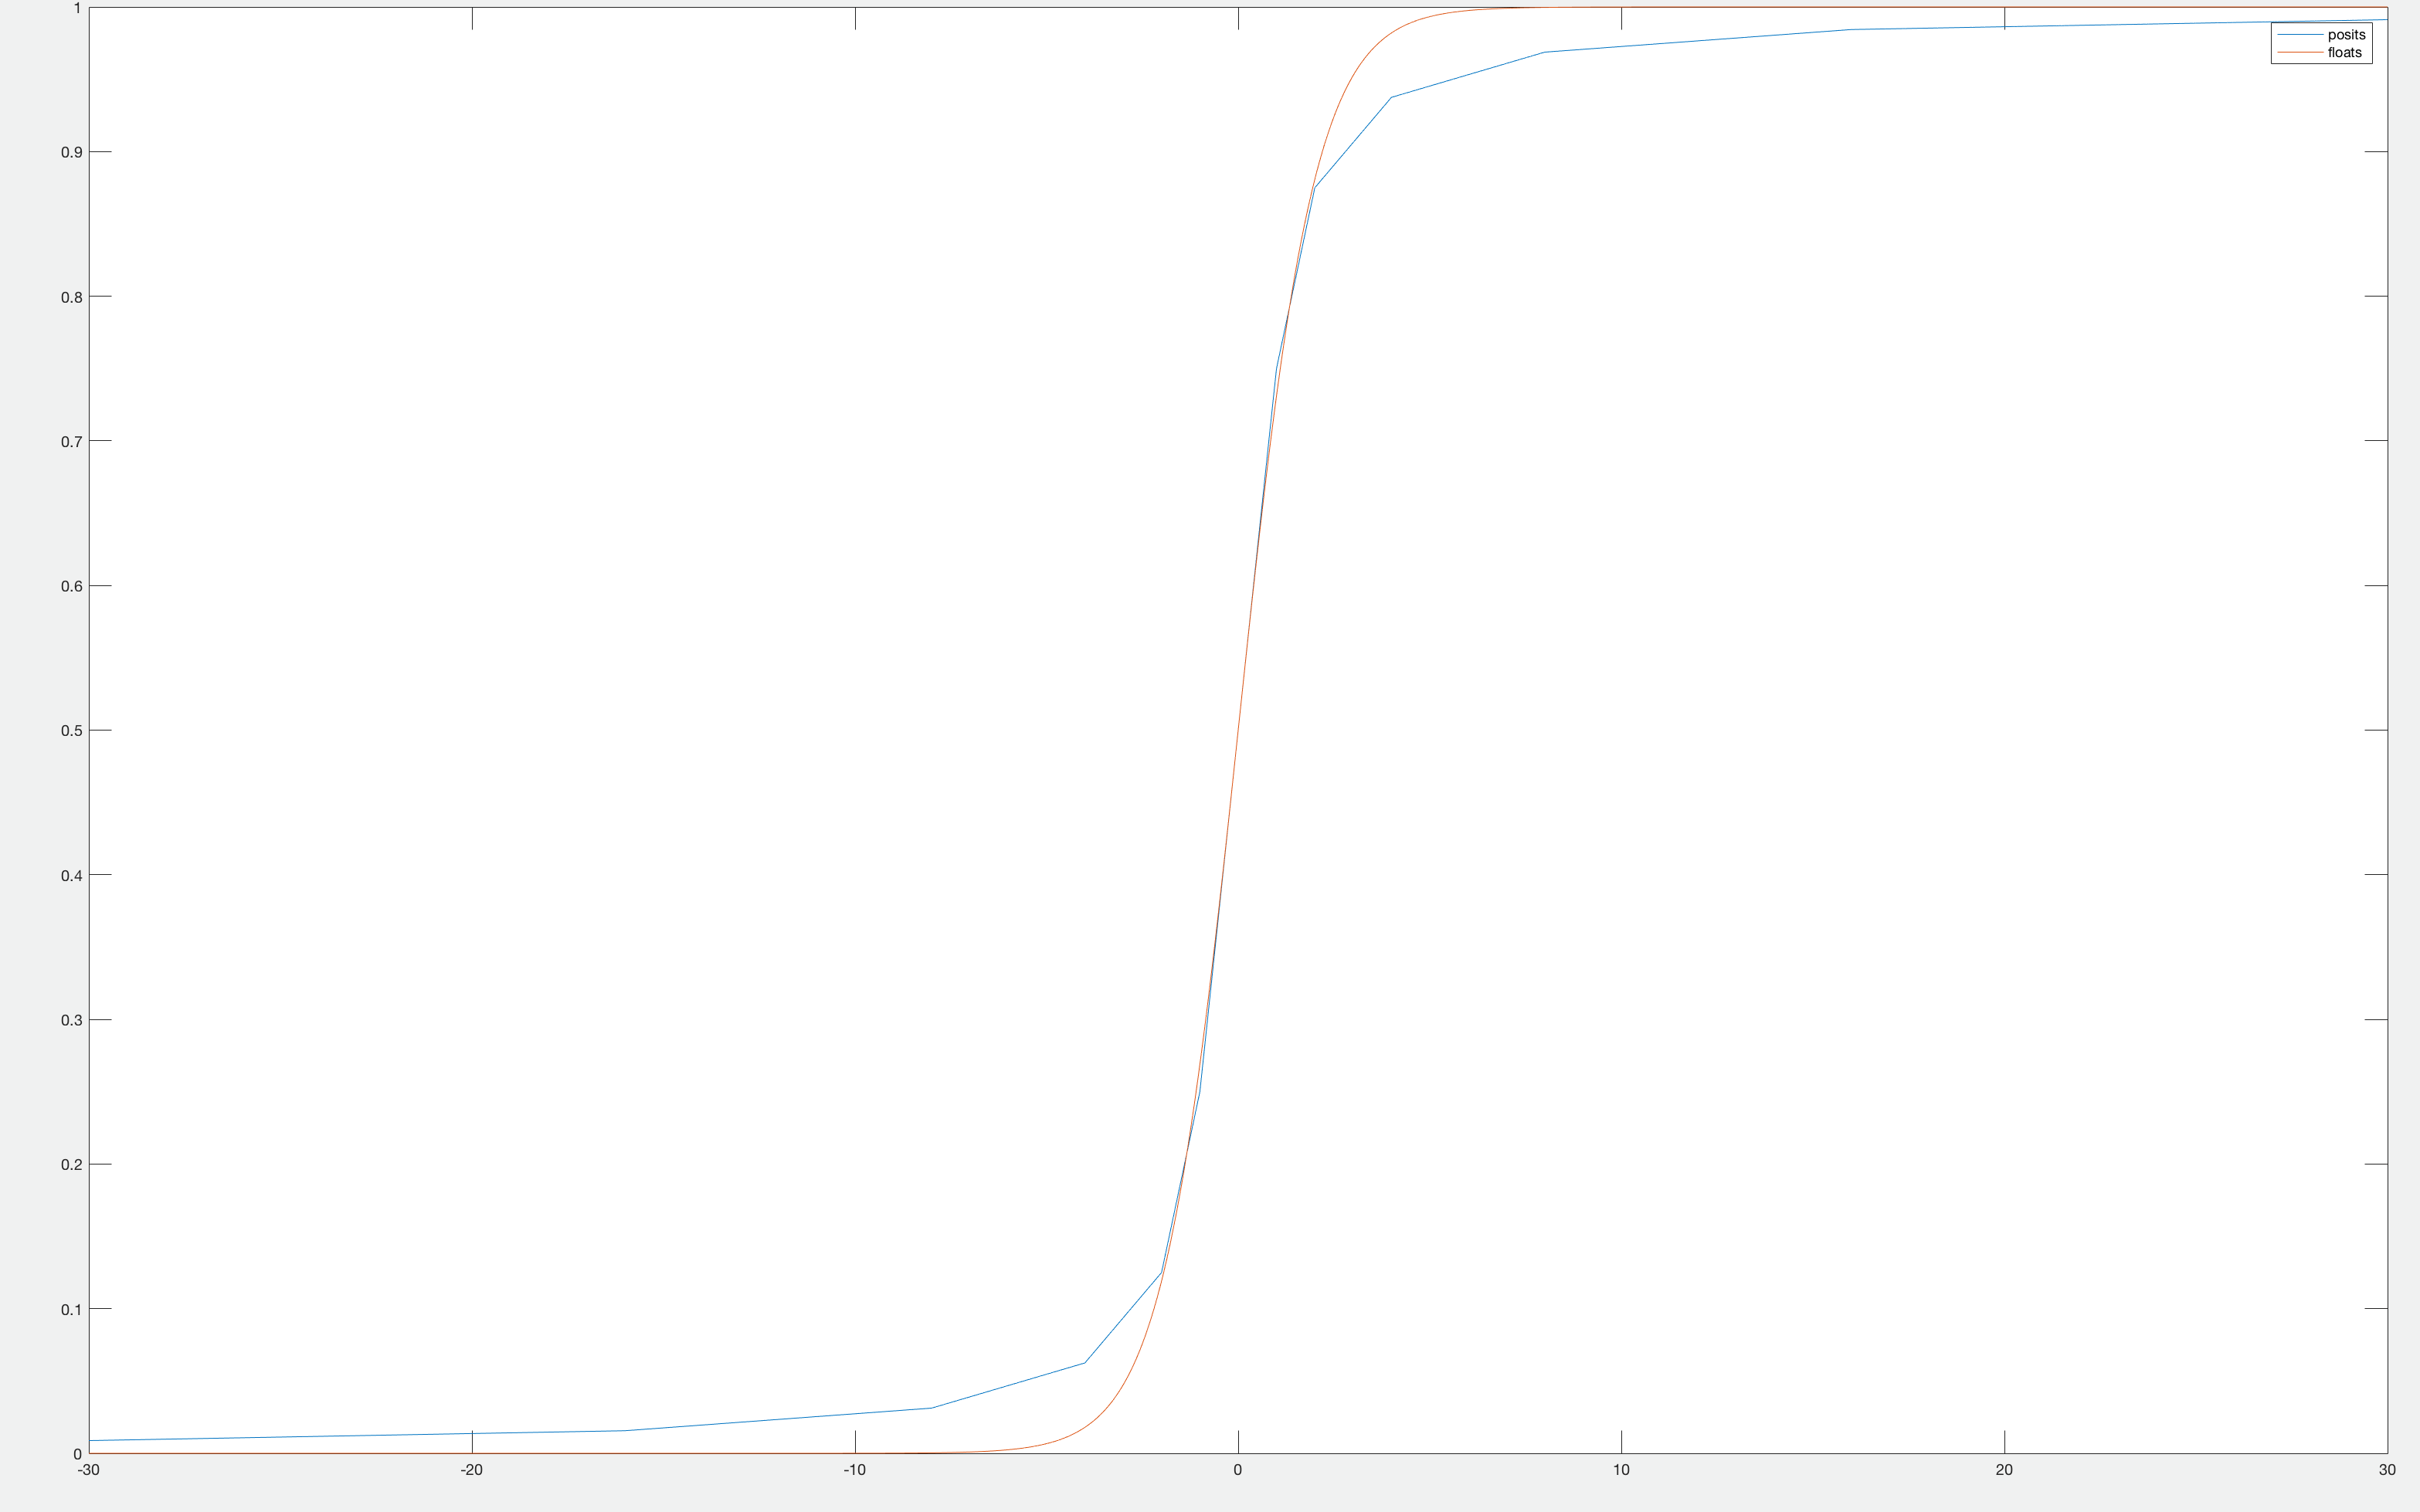
\includegraphics[scale=0.15]{sigmoide_2}
	\centering
	\caption{"Sigmoide"}
\end{figure}

\subsubsection{Conclusioni}
Come si può evincere dalla figura, il grafico ottenuto con i  Posit sembra essere una spezzata che segue l'andamento della sigmoide con i Float, inoltre i due grafici si vanno a sovrapporre nell'origine. In generale comunque possiamo affermare che effettivamente questo tipo di manipolazione sui bit, ha fornito una approssimazione della sigmoide.

\subsubsection{Codice}

\begin{lstlisting}[language=C++]
//Sigmoide con Float
float sigmoid(float &x){
	return 1/(exp(-x)+1);
}

//Sigmoide con Posit
unsigned int sigmoid(unsigned int bits){
	bits = bits ^ 0x80000000;
	bits = bits >> 2;
	return bits;
}


//Conversione da Posit[32-0] a Float
float Posit::subconv(){
	union {
		float f;
		uint32_t bits;
	};
	bits=0;
	
	if((mBits & 0xFFFFFFFF) == 0)
	return 0.0f;
	signed char c = (signed char)(regime());
	c+= 127;
	unsigned int esponente = (unsigned int)(c);	
	
	esponente = esponente<<23;
	bits = bits | esponente;
	unpacked_t aup = unpack_posit(mBits, mNbits, mEs);
	unsigned int fr_ = aup.frac;
	
	fr_ = fr_>>9;
	bits = bits | fr_;
	int segno = aup.neg;
	if(segno == 0)
		bits &= 0x7FFFFFFF;
	else
		bits |= 0x80000000;
	
	return f;
}
\end{lstlisting}
\newpage
\subsection{Tempi}

Una volta dimostrato che possiamo approssimare la sigmoide, il passo successivo è quello di provare che effettivamente vi sia risparmio tangibile nell'eseguire i calcoli. \\
Questo test, suddiviso in più parti, effettua diversi confronti, sui tempi di elaborazione, fra sigmoide su Posit e sigmoide ottenuta in vari modi sui Float.

\subsubsection{Parte 1}

Il primo confronto eseguito è stato con la funzione sigmoide esponenziale  $ f(x) = \frac {1}{1 + e^{-x}} $, la stessa utilizzata nel test numerico.\\
Esso consiste nel generare un milione di Float pseudo-casual,i e di scriverli su file sia come Float che come Posit sotto forma di bit, il tutto per evitare di falsare il test a sfavore di questi ultimi, in quanto nel tempo di elaborazione vi sarebbe anche il tempo di conversione. \\
Una volta acquisiti i dati da file, per ciascun tipo, impiego la funzione clock\_gettime(), la quale viene richiamata prima e dopo aver finito di calcolare la sigmoide su tutti i dati.\\
Successivamente ho ripetuto lo stesso esperimento, incrementando gradualmente il numero di elementi, per verificare se l'eventuale margine fosse influenzato dalle dimensioni, nello specifico lo step scelto è stato di 10 mila, con numero massimo di 5 milioni.

\begin{figure}[h]
	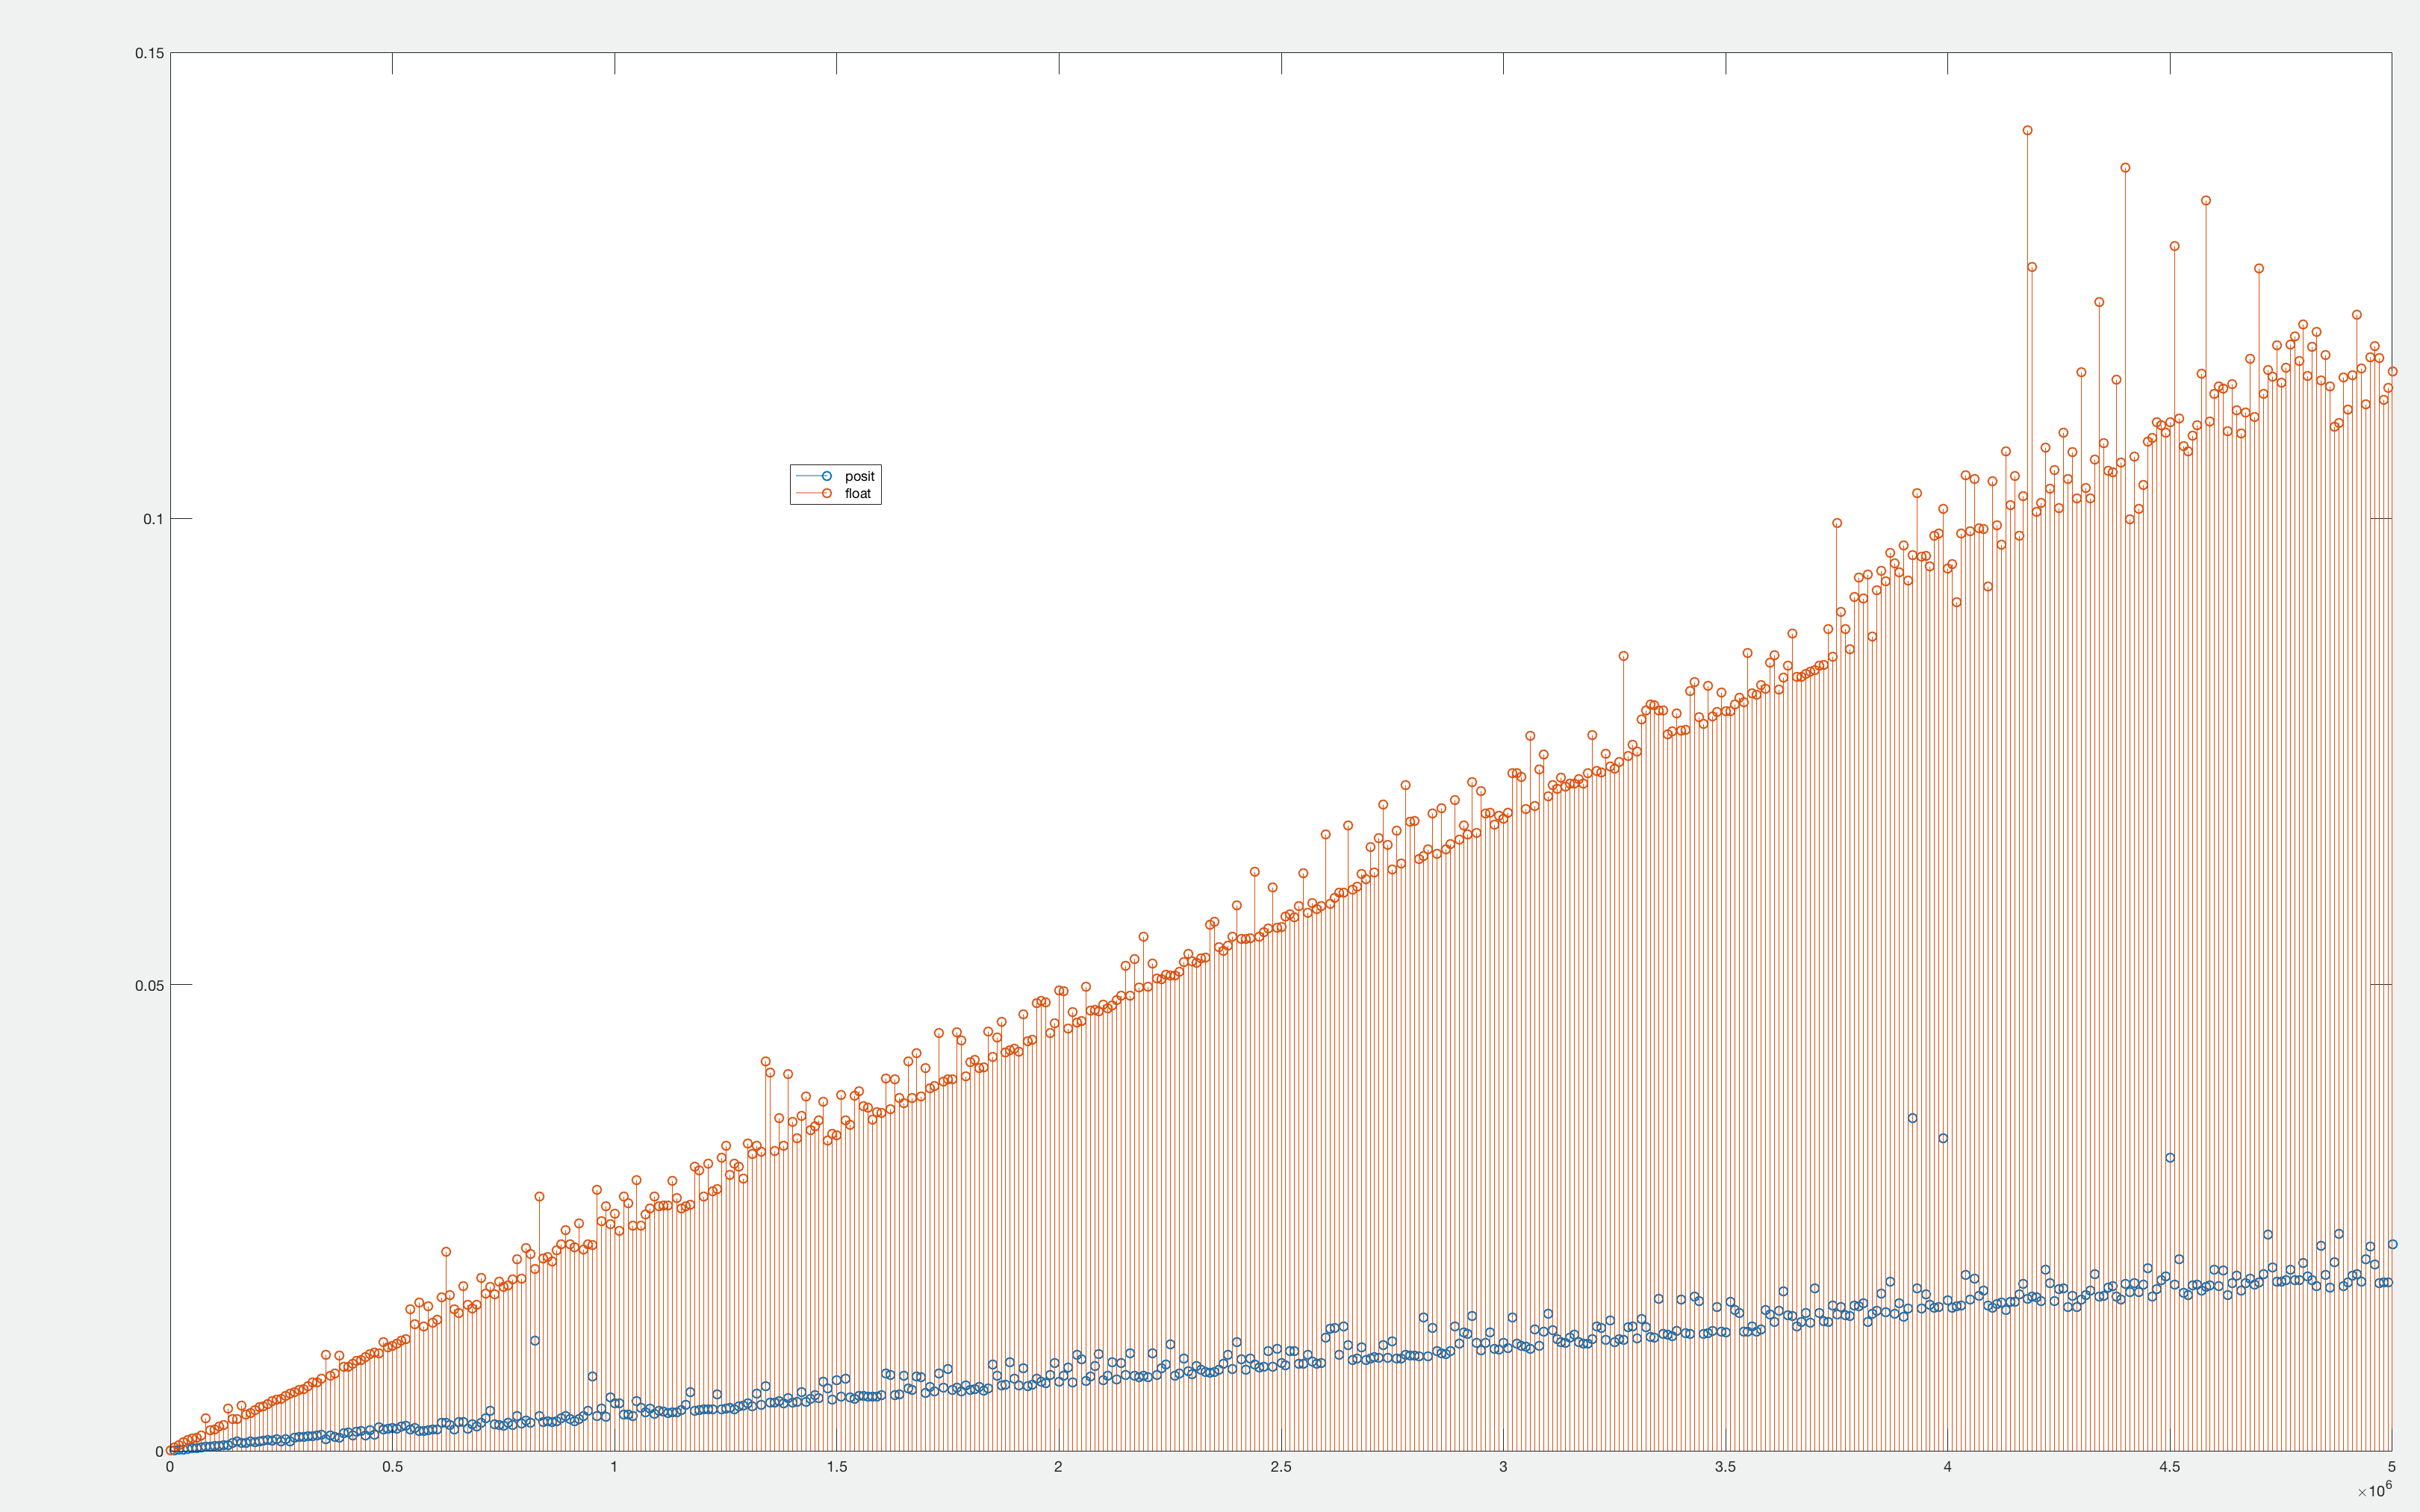
\includegraphics[scale=0.15]{tempi}
	\centering
	\caption{"Tempi all'aumentare degli elementi"}
\end{figure}


\subsubsection{Parte 1 - Esito}


I risultati hanno evidenziato che la funzione, calcolata mediante manipolazione di bit, quindi impiegando solamente la ALU del processore, è più rapida di $\approx1.5-1.8$\ volte su un campione di 1 milione di elementi. \\
Per quanto riguarda l'incremento, come si può evincere dalla Figura 3, il tempo di elaborazione aumenta linearmente all'aumentare del numero degli elementi in entrambi i casi, di conseguenza possiamo affermare che il vantaggio rimane pressoché costante.

 
\subsubsection{Parte 2}

In questa seconda parte ho voluto usare come metro di paragone, invece della curva logistica su Float, una sua versione approssimata ottenuta mediante quanto descritto nell'articolo "A Fast, Compact Approximation of the Exponential Function"\cite{afast}. In particolare si sfrutta il fatto che, i Float, utilizzano una rappresentazione del tipo $2^x$ per ottenere $e^x$, il tutto operando semplici operazioni sui bit ed una divisione come fattore correttivo. %controllare

\subsubsection{Parte 2 - Esito}

%Aggiungere codice sigmoide approssimata, clockgettime per il test

I risultati mostrano che, nonostante l'aver adoperato questo tipo di approssimazione, risulta essere ancora conveniente l'utilizzo dei Posit.
%aggiungere vantaggio

\subsubsection{Parte 3}

Test con x/boh

\subsubsection{Parte 3 - Esito}

\subsubsection{Codice}

\newpage
\section{Divisione e Moltiplicazione mediante Regime}
\subsection{Introduzione}

Lavorando con Posit con 0 bit di esponente, il "superesponente" $(2^{2^{es}})^{regime}$ viene notevolmente semplificato, in quanto $2^{2^{0}} = 2 => 2^{regime} $ esattamente come nei Float. L'unica differenza consiste nel fatto che il regime non è un campo a dimensione fissa.\\ L'idea è stata quella di sfruttare questa caratteristica dei Posit 0, per implementare moltiplicazioni e divisione, per potenze del 2, semplicemente intervenendo sul regime. Il grande vantaggio consiste nel fatto che essendo esso composto da una sequenza di bit uguali, incrementarne o decrementarne il valore è relativamente semplice e poco costoso!\\
Ad esempio, dato un Posit-0: 0 001 00000\footnote{Regime = -2; Mantissa = 0}, il quale rappresenta +0.25, se volessimo dividerlo per 2, basterebbe aggiungere uno 0 al regime, ottenendo quindi 0 0001 0000\footnote{Regime = -3; Mantissa = 0} = +0.125

\subsection{Accuratezza}

Dopo aver implementato le funzioni che eseguono rispettivamente moltiplicazione e divisione, ne ho voluto testare l'accuratezza confrontando i risultati, utilizzando come riferimento i Double. \\
Nello specifico ho confrontato il delta fra il riferimento e i risultati ottenuti eseguendo lo stesso calcolo su Posit e Float.

\subsubsection{Risultati} 

Su un campione di 1 milione di numeri non è stata evidenziata alcuna differenza fra i risultati ottenuti con i Float e con i Posit nel 100\% dei casi.\\
Il risultato è giustificabile con il fatto che, eliminando il "superesponente" il Posit diventa un Float con una mantissa a dimensione variabile.

\subsection{Tempi}
Una volta dimostrato che non vi è alcun vantaggio, in termini di accuratezza, ho voluto verificare quanto fosse il guadagno in termini computazionali.\\
Il test è stato svolto su un campione di 1 milione di elementi, sfruttando la funzione clock\_gettime(), come già fatto in precedenza.
\subsubsection{Risultati}

\subsection{Codice}
\begin{lstlisting}[language=C++]
//Prova.cpp
printf("Ciao");


\end{lstlisting}

\newpage
\section{Conclusioni}
Nel complesso i Posit si sono rivelati un'ottima alternativa alle soluzioni attualmente impiegate, % aspetti positivi, 
L'unica cosa che 

\newpage




	\nocite{articolo1}
	
	\printbibliography[title=Bibliografia]

	

\end{document}